%%%%%%%%%%%%%%%%%%%%%%%%%%%%%%%%%%%%%%%%%%%%%%%%%%%
%
%  New template code for TAMU Theses and Dissertations starting Fall 2016.
%
%  Author: Sean Zachary Roberson
%	 Version 3.16.09
%  Last updated 9/12/2016
%
%%%%%%%%%%%%%%%%%%%%%%%%%%%%%%%%%%%%%%%%%%%%%%%%%%%
%%%%%%%%%%%%%%%%%%%%%%%%%%%%%%%%%%%%%%%%%%%%%%%%%%%%%%%%%%%%%%%%%%%%%%
%%                           SECTION III
%%%%%%%%%%%%%%%%%%%%%%%%%%%%%%%%%%%%%%%%%%%%%%%%%%%%%%%%%%%%%%%%%%%%%



\chapter{RESULTS}

The results of this research are split into the testing of features and learning algorithms, as detailed in the preceding testing methodology.

\section{Feature Evaluation}
As stated previously, plots of the various distances metrics for features are plotted in order to evaluate whether a feature is sufficient.
The average extraction time for each feature for a single image is also shown.
These features were extracted using a single core of an Intel i5 processor with a maximum clock speed of 2.7 GHz.
Shown below are the plots and average extraction time for pixel distribution, BRIEF descriptors, and blob detection.

\subsection{Pixel Distribution}
Below are figures showing the MSEs (figure 3.1), EMDs (figure 3.2), and Bhattacharyya (figure 3.3) distances between consecutive image pairs.



\begin{figure}[htb]
\centering
\scalebox{1.0}{% This file was created by matplotlib2tikz v0.6.11.
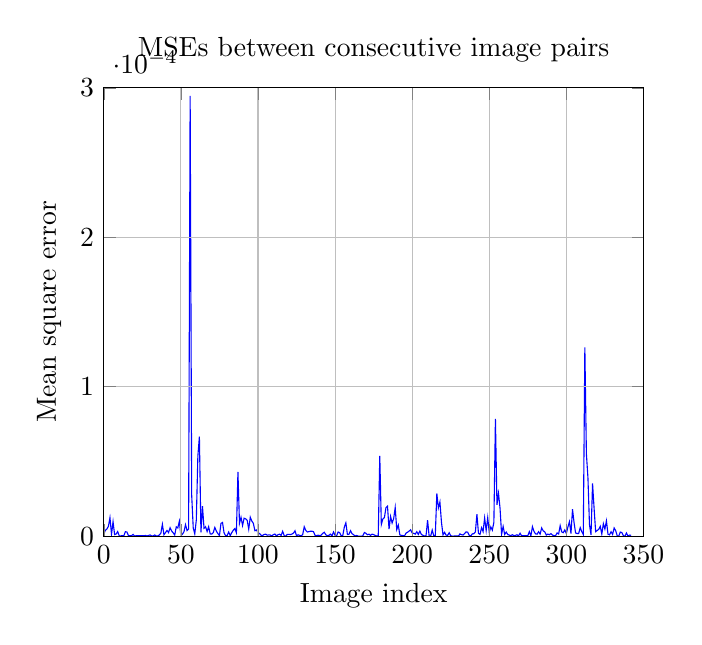
\begin{tikzpicture}

\begin{axis}[
title={MSEs between consecutive image pairs},
xlabel={Image index},
ylabel={Mean square error},
xmin=0, xmax=350,
ymin=0, ymax=0.0003,
axis on top,
tick pos=both,
xmajorgrids,
ymajorgrids
]
\addplot [blue, forget plot]
table {%
0 1.30759662845069e-06
1 3.93114240529637e-06
2 4.78311378198365e-06
3 6.65946113359597e-06
4 1.24077329101662e-05
5 1.25434088727666e-06
6 9.68247821761502e-06
7 1.0676233511832e-06
8 1.49782370879418e-06
9 3.08474963013497e-06
10 2.68073390341467e-07
11 2.15237629082468e-07
12 3.81678782610429e-07
13 3.08895074865884e-07
14 2.99493741347558e-06
15 2.79284352954063e-06
16 3.48476020412313e-07
17 4.1545293190413e-07
18 3.73995883597268e-07
19 1.20518764273988e-06
20 1.07109914016393e-07
21 3.20920172250933e-07
22 2.8085928513772e-07
23 3.64524979765216e-07
24 2.7590271913343e-07
25 2.93994017152323e-07
26 3.16823434291614e-07
27 4.95293751979868e-07
28 1.74750149663952e-07
29 4.34443851312002e-07
30 8.64332277948658e-07
31 1.89479409406583e-07
32 2.57723085168335e-07
33 7.79867886255185e-07
34 1.8917808516158e-07
35 8.44455272373226e-08
36 8.26396389553944e-07
37 1.94614169498285e-06
38 7.94661447612775e-06
39 9.76222360299693e-07
40 2.38804105255339e-06
41 3.8393692786081e-06
42 2.42249829591148e-06
43 5.64849718163411e-06
44 3.47353857941925e-06
45 2.20281484329866e-06
46 8.05509028335412e-07
47 6.2817653382404e-06
48 5.51249993344148e-06
49 1.001113225292e-05
50 2.54924688488245e-07
51 1.34886364556021e-06
52 2.99947110729085e-06
53 7.72635521781113e-06
54 3.76198949395782e-06
55 4.88569132673244e-06
56 0.000294571003586882
57 2.74405727939059e-05
58 5.52318249311712e-06
59 1.58609503155781e-06
60 1.07384854461998e-05
61 5.34878452877618e-05
62 6.66874062632107e-05
63 2.50164557041393e-06
64 2.00817707615594e-05
65 5.30368463757137e-06
66 6.33780213279857e-06
67 3.13141904253927e-06
68 6.35031278038191e-06
69 1.50552532221708e-06
70 1.45102598083516e-06
71 2.39596396374206e-06
72 5.86375327159961e-06
73 3.37677606277996e-06
74 1.75413174761666e-06
75 4.01358202927642e-07
76 8.57500607251294e-06
77 9.17767533618542e-06
78 2.20473962835967e-06
79 3.70493717491627e-07
80 4.53318034609159e-07
81 2.76946776236097e-06
82 3.80093216275175e-07
83 2.34975823097759e-06
84 4.03710576291713e-06
85 5.05913869063886e-06
86 2.31987892960509e-06
87 4.29454564220376e-05
88 8.61723574085368e-06
89 1.2644585284094e-05
90 7.17996252804166e-06
91 1.20271895442986e-05
92 1.15865590361257e-05
93 1.06476482055667e-05
94 4.70590126286778e-06
95 1.27168222433991e-05
96 1.01074803672317e-05
97 8.59111825314659e-06
98 3.68600106384191e-06
99 4.19937307532463e-06
100 2.24189401293794e-06
101 1.82566339563992e-06
102 6.42139071391689e-07
103 4.52038764746652e-07
104 1.16001230457591e-06
105 1.37834512214694e-06
106 6.76074499885242e-07
107 8.91340710222722e-07
108 7.73525543303954e-07
109 2.31897018642889e-07
110 1.05137053566674e-06
111 1.45228271269136e-06
112 2.05780156991548e-07
113 1.02069658330745e-06
114 1.36787808603711e-06
115 4.77431067782972e-07
116 3.28038743593627e-06
117 3.37552134361531e-07
118 6.86684209439491e-08
119 1.1658672346837e-06
120 1.24028951654004e-06
121 1.10606230381462e-06
122 1.3951847071035e-06
123 2.05859109862811e-06
124 3.62670533359051e-06
125 2.25211535063055e-07
126 9.25817050867611e-07
127 5.57263852614496e-07
128 2.21824226900935e-07
129 1.076885804327e-06
130 6.29854798834356e-06
131 3.92198225793739e-06
132 2.78881032847696e-06
133 3.04221007972956e-06
134 3.29869523023565e-06
135 3.32291754893959e-06
136 3.01868797072934e-06
137 6.00147687105669e-07
138 3.40976400507821e-07
139 7.19497347664502e-07
140 3.50274631960524e-07
141 7.13384229068955e-07
142 1.88735503599875e-06
143 2.63699040127297e-06
144 9.4246092873315e-07
145 3.05001541144318e-07
146 5.79871485630672e-07
147 1.41435256745252e-06
148 1.68548958996932e-07
149 2.84335759675337e-06
150 5.92754920944572e-07
151 2.80078453943133e-07
152 2.82514898313416e-06
153 2.32962671046456e-06
154 1.26116821128461e-07
155 4.98433157594667e-07
156 6.09571944094366e-06
157 8.92669932606319e-06
158 1.16951638418767e-06
159 1.25565608549449e-06
160 3.67692317813635e-06
161 1.72017519362271e-06
162 1.01551704833077e-06
163 7.42546696629789e-08
164 4.74375486373901e-07
165 4.43824411680302e-08
166 5.62595255259011e-08
167 1.69313461002377e-08
168 2.19754450437096e-07
169 2.4727801947544e-06
170 1.9201148301363e-06
171 9.82580463298493e-07
172 1.30722145032552e-06
173 5.78803331073788e-07
174 1.34507833669583e-06
175 1.07600439029435e-06
176 4.99528755123417e-07
177 1.69575405824516e-07
178 6.99612932900588e-08
179 5.36712281509406e-05
180 7.80254259395102e-06
181 1.15233921756347e-05
182 1.24366209842265e-05
183 1.91449015556524e-05
184 2.01289362791512e-05
185 4.71623153425753e-06
186 1.32327157797085e-05
187 8.83746881865793e-06
188 1.17717968817386e-05
189 1.91829621015737e-05
190 4.38924349016613e-06
191 7.43645523260865e-06
192 8.84240803619226e-07
193 4.65745127035512e-07
194 4.13946724600262e-07
195 1.17276464071539e-07
196 2.03196583833132e-06
197 2.63944245978362e-06
198 3.40203610766265e-06
199 4.29224168571333e-06
200 2.17882972210646e-06
201 1.91634099723564e-06
202 1.38348628145953e-06
203 3.01608239921431e-06
204 1.18014681049519e-06
205 3.42602386760215e-06
206 1.07995368436807e-06
207 5.93656094537842e-07
208 1.28427639396654e-07
209 3.23321716859936e-07
210 1.07052168084515e-05
211 7.66113400459289e-08
212 9.53534514539772e-08
213 4.1173439214213e-06
214 2.5835433560941e-07
215 5.86274043760366e-07
216 2.86081190479712e-05
217 1.89334649696118e-05
218 2.29311341626776e-05
219 9.40083145784835e-06
220 8.8405477710896e-07
221 2.59176039447387e-06
222 7.13893791867627e-07
223 5.78541256901291e-07
224 2.31602552553846e-06
225 2.98404191724128e-07
226 7.49221330301629e-08
227 7.45315259943407e-08
228 2.07403855812218e-07
229 1.4500402741962e-07
230 6.85082903752725e-08
231 1.55868511129584e-06
232 1.04215419851243e-06
233 7.90178082469437e-07
234 1.83183022567795e-06
235 2.88148419931531e-06
236 2.70122143750389e-06
237 5.6745768007305e-07
238 9.26400586548779e-08
239 1.5827947606643e-06
240 1.67249151919451e-06
241 2.8730899354236e-06
242 1.47492172248248e-05
243 1.92117215030723e-06
244 1.20166942684187e-06
245 5.68532300595608e-06
246 3.06219974429243e-06
247 1.22577393841412e-05
248 3.79770307594703e-06
249 1.24175095982436e-05
250 2.54394445154402e-06
251 6.23179028948976e-06
252 4.04067957877285e-06
253 9.28599792532623e-06
254 7.84910569588343e-05
255 2.09261553465492e-05
256 2.86000240697629e-05
257 1.8656442919746e-05
258 1.27996481023729e-06
259 6.51498191162116e-06
260 1.16231886980434e-06
261 2.75237951427698e-06
262 1.12598865913848e-06
263 7.21827734054791e-07
264 3.97081652449237e-07
265 9.91298330740796e-07
266 3.32223003109296e-07
267 5.54763468810254e-07
268 9.47916388718618e-07
269 2.56021398430069e-07
270 1.9811320429047e-06
271 1.98548716596431e-07
272 3.65561122695605e-07
273 3.2044834871259e-07
274 4.04194928705693e-07
275 3.44283501100209e-07
276 3.01693174988031e-06
277 1.80245221902927e-07
278 6.37259573882653e-06
279 3.27519961736268e-06
280 1.51466483560701e-06
281 1.34426609406041e-06
282 3.00861872318718e-06
283 1.38992192741069e-06
284 5.51639276867111e-06
285 3.55599346674151e-06
286 2.94825243246224e-06
287 7.28854604272379e-07
288 1.39461045877801e-06
289 9.69930572642221e-07
290 1.67598298543857e-06
291 7.41835202400883e-07
292 3.98625800799992e-07
293 3.82142896867461e-07
294 2.16018451998631e-06
295 1.50633557803101e-06
296 7.01738544222381e-06
297 2.8912848016868e-06
298 2.3471628729668e-06
299 4.22688335594204e-06
300 1.77137195132673e-06
301 6.08799698659116e-06
302 9.70438938173983e-06
303 1.71256978582177e-06
304 1.80541180229435e-05
305 9.04382352924181e-06
306 2.13410893662108e-06
307 1.78913260913557e-06
308 1.82916281434397e-06
309 5.72470748900539e-06
310 3.07667536350588e-06
311 1.15791094592876e-06
312 0.000126373774879095
313 5.51237220513738e-05
314 3.92688701705387e-05
315 7.70206941912572e-06
316 9.09697104038464e-07
317 3.53006085639613e-05
318 1.85722003742639e-05
319 3.02819362324145e-06
320 3.80282187834382e-06
321 4.60626754081911e-06
322 6.5992973693129e-06
323 1.38934278446767e-06
324 8.33994090143177e-06
325 4.77285344257123e-06
326 1.02685705862111e-05
327 1.37036764062941e-06
328 8.89416380474965e-07
329 3.0142346293562e-06
330 1.18753632737531e-06
331 5.51264590273301e-06
332 3.67086903812985e-06
333 2.82015563506219e-07
334 6.59402925521138e-08
335 2.75582505079607e-06
336 2.39918390288949e-06
337 2.9951027697987e-07
338 2.32643240855799e-08
339 2.13503309318589e-06
340 6.26284680846664e-08
341 7.5103577433361e-07
342 5.94890174559421e-07
};
\end{axis}

\end{tikzpicture}}
\caption{Plot of MSEs between distributions of consecutive image pairs.}
\label{fig:tamu-fig3}
\end{figure}

\begin{figure}[htb]
\centering
\scalebox{1.0}{% This file was created by matplotlib2tikz v0.6.11.
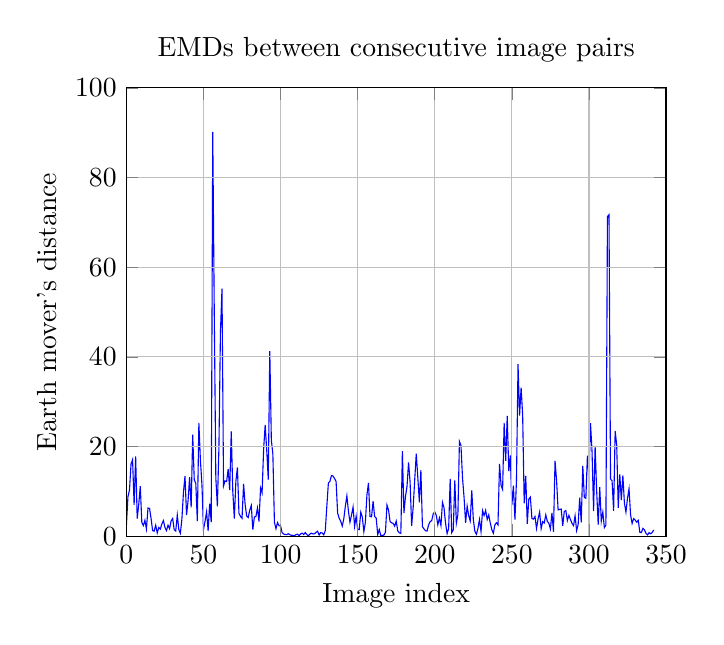
\begin{tikzpicture}

\begin{axis}[
title={EMDs between consecutive image pairs},
xlabel={Image index},
ylabel={Earth mover's distance},
xmin=0, xmax=350,
ymin=0, ymax=100,
axis on top,
tick pos=both,
xmajorgrids,
ymajorgrids
]
\addplot [blue, forget plot]
table {%
0 2.3778796290152
1 8.79615940584014
2 10.287308314995
3 16.0845824924402
4 17.0695109855852
5 7.01164415064003
6 17.7849437311351
7 3.91473494013
8 7.09571080950003
9 11.14904367603
10 3.05856918837006
11 2.37154563633017
12 3.55681191739503
13 1.61446631067008
14 6.29461871920512
15 6.19645124349012
16 3.943596547245
17 1.24111686072003
18 1.13740070307003
19 2.43127985757
20 0.72852418468517
21 1.93865587071026
22 1.5840062123402
23 2.74321373103009
24 3.47725463442008
25 1.97087706151517
26 1.24413553363511
27 2.45622644866534
28 1.67047682785534
29 3.41880869383529
30 3.95323812937506
31 1.42712864842523
32 1.15437963046526
33 4.72056592696508
34 1.48416509742006
35 0.65254032712517
36 3.84380763592517
37 9.77713027170006
38 13.41056019927
39 4.69480092306026
40 7.9485636117152
41 13.1769038313602
42 6.44908974255026
43 22.6539079854752
44 12.5784964503002
45 11.8081447790702
46 3.34070094382511
47 25.275193967835
48 16.929180354585
49 11.4789676110451
50 1.49215636290011
51 3.30864531712509
52 5.42674659447003
53 1.21747055721006
54 7.23431518204506
55 3.14663409831006
56 90.1614606690751
57 49.45315858875
58 12.9767208047251
59 6.66886579414503
60 19.6674697370101
61 45.5861520715501
62 55.19475554676
63 11.20354448025
64 12.3384751995151
65 12.1991487572401
66 14.97758277054
67 10.2994331503651
68 23.3524280648701
69 10.0209103400401
70 3.91536361381506
71 12.2291863060351
72 15.358488012015
73 5.08152836865026
74 4.40249618154012
75 4.00921430418017
76 11.6902093086151
77 7.08304596114014
78 4.48769368864514
79 4.15142340466534
80 5.83631213764523
81 6.85543652655023
82 1.45271983107
83 4.28734728453023
84 4.38249670621503
85 6.30896269870508
86 3.24468310969511
87 10.7581844815054
88 9.66996306390046
89 19.4002694473953
90 24.8245182877951
91 19.2667421883452
92 12.6312797871903
93 41.2618048069652
94 21.4825910015401
95 18.2738852487157
96 3.11285492457052
97 1.65755474773512
98 3.03382108927506
99 2.31111415431006
100 2.29336040431506
101 0.778975936980114
102 0.485432300655001
103 0.374899363410114
104 0.335486514960114
105 0.566752619460114
106 0.314020405605
107 0.218006442630114
108 0.186817673895057
109 0.112905652320057
110 0.355333977390057
111 0.437612573955057
112 0.101739812535057
113 0.523300237470114
114 0.670459683300057
115 0.376072716075114
116 0.807729307560114
117 0.3857104653
118 0.102506190045
119 0.463285218900001
120 0.677478582015057
121 0.496301973750057
122 0.554399978820057
123 0.864257270745114
124 1.10331457486511
125 0.268537951785
126 0.801975638520001
127 0.707012344650114
128 0.295453116615
129 1.28195333056506
130 6.70861237894512
131 11.8684802393101
132 12.2279120524201
133 13.526243657625
134 13.410179019405
135 12.8651307252001
136 12.1843578040501
137 5.13235606515017
138 4.01842145173517
139 3.31929690886514
140 2.26175280904508
141 3.87918518613
142 6.68212254595511
143 8.99451634279511
144 5.59090779555006
145 3.13072225870509
146 4.710773043645
147 6.49103593032003
148 2.19599088429014
149 4.45937133130543
150 1.46418873096006
151 1.45275788242517
152 5.35168333102506
153 4.29363421875006
154 1.00185795640506
155 3.10521079084511
156 9.19010171713512
157 11.8917728664901
158 4.40446707246
159 4.33517054604023
160 7.79568623152501
161 4.37086822350023
162 4.058176520385
163 0.35838950367017
164 1.50475627908006
165 0.150225237135057
166 0.186545012595
167 0.232071317745227
168 0.894289688430171
169 6.95182396864512
170 5.85723944271012
171 3.30083314069529
172 2.981961268545
173 2.86324659076506
174 2.23424263716006
175 3.36354819973517
176 1.20167645493017
177 0.761868231780171
178 0.626229091800057
179 18.9876548615701
180 5.15842726974
181 8.81763928851018
182 11.1251201770653
183 16.4662903839001
184 12.0542410113901
185 2.29266392613017
186 6.45139695067529
187 12.6356620858651
188 18.4264569407701
189 13.1253056765852
190 7.57299811104026
191 14.7455780284501
192 2.14205376726
193 1.63107396112511
194 1.19821733250023
195 1.16115233764517
196 2.53026603832506
197 3.27533885065512
198 3.45176903707517
199 4.99094269522523
200 5.41839399985506
201 4.63933770982517
202 2.53541963167512
203 4.05704675002512
204 2.40289968790506
205 7.55200541199009
206 6.3194900049752
207 2.86076265795023
208 0.605281620570171
209 1.70007826315506
210 12.7544796987303
211 0.805013688375058
212 1.40612625147011
213 12.4553294638503
214 2.87895376813506
215 4.83026657940014
216 21.1339938082051
217 20.2268472768155
218 12.9806866947752
219 8.64331877166011
220 2.96771779780509
221 6.68120534512514
222 4.58055989133009
223 3.40212010026014
224 10.2344104994253
225 3.77069607516006
226 1.08033210240026
227 0.428794220820028
228 1.72138091955017
229 3.71264177148034
230 1.02803920803014
231 5.70819234280549
232 4.61611923358535
233 5.7677503835252
234 3.73168934149549
235 4.74603117250523
236 2.929828640655
237 1.461522088605
238 0.666134057865057
239 2.56062234910506
240 2.99584576354506
241 2.53768914978017
242 16.1283555711002
243 11.3476871952452
244 10.4213280922651
245 25.2617378052602
246 16.8056030733903
247 26.8299277382252
248 14.5279435423351
249 18.0177476980501
250 6.94351659241506
251 11.2746954946801
252 3.68619744579009
253 12.46331454966
254 38.37033824085
255 26.9056338416251
256 33.1463840773051
257 27.0525170304002
258 7.34999015731514
259 13.457440344045
260 2.77877023615511
261 8.29573494832512
262 8.73429730191
263 3.95197827102006
264 3.81410238885011
265 4.38576656407506
266 1.71849671910028
267 3.85859027050511
268 5.3503857189002
269 1.67540596867517
270 3.25167176235014
271 2.94833799900011
272 4.7481343587
273 3.31844700534012
274 2.8903953468152
275 1.61044023424514
276 5.2008990635102
277 0.997733564220056
278 16.8073861264651
279 12.4542993803852
280 5.86439705250012
281 5.979543081525
282 6.05855616109523
283 2.30448270897034
284 5.51057470567517
285 5.71791453171012
286 3.49458663609012
287 4.6496465333702
288 3.71482945192503
289 2.88872130114006
290 2.35319375680511
291 4.55707817094006
292 1.248837412845
293 2.61882040852512
294 8.58734710576512
295 3.08464549270512
296 15.7067487405001
297 8.64501847339503
298 8.46474820168508
299 17.9691212173951
300 13.2022804197751
301 25.2286056302701
302 18.9598561056751
303 5.60519337342011
304 20.130462070305
305 10.0583659015651
306 2.58307534263006
307 10.9425575777551
308 3.36048056452506
309 5.37193818706509
310 1.91881712494503
311 2.46564313584
312 71.2984242702752
313 71.6944595866352
314 12.7693641142651
315 12.3505548662252
316 5.63628431064003
317 23.4618008064301
318 20.2999839030601
319 6.320221693305
320 13.7984109035401
321 8.06790628182
322 13.540068013935
323 7.36798657500026
324 5.37762326875526
325 8.47072506432006
326 10.5618663259051
327 4.72716487969514
328 2.8332342339302
329 3.92912784852006
330 3.61686390459011
331 3.11430927117012
332 3.5352989071652
333 0.878926677420199
334 0.810756285060114
335 1.74879789811511
336 1.42249709872506
337 0.60864546939
338 0.273112150710057
339 0.784092503055
340 0.542942678115057
341 0.827316717165114
342 1.38769133757
};
\end{axis}

\end{tikzpicture}}
\caption{Plot of Earth mover's distances between distributions of consecutive image pairs.}
\label{fig:tamu-fig3}
\end{figure}

\begin{figure}[htb]
\centering
\scalebox{1.0}{% This file was created by matplotlib2tikz v0.6.11.
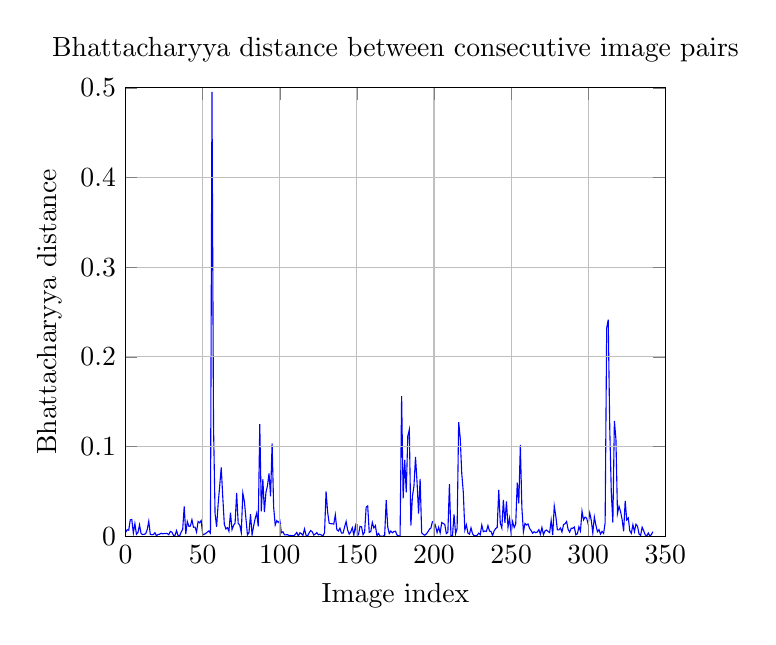
\begin{tikzpicture}

\begin{axis}[
title={Bhattacharyya distance between consecutive image pairs},
xlabel={Image index},
ylabel={Bhattacharyya distance},
xmin=0, xmax=350,
ymin=0, ymax=0.5,
axis on top,
tick pos=both,
xmajorgrids,
ymajorgrids
]
\addplot [blue, forget plot]
table {%
0 0.00424250907761757
1 0.00720453297702217
2 0.00667518225733314
3 0.0182084090537029
4 0.0186253620268533
5 0.00349784272727805
6 0.0140082288139858
7 0.00212250526550013
8 0.00416678704858617
9 0.0125920420453202
10 0.00296671064930827
11 0.00185830794139257
12 0.00210625762149454
13 0.00273762674861986
14 0.00743607926482914
15 0.0166529796861671
16 0.00207260123325636
17 0.00158530354202563
18 0.00181543134853952
19 0.00392770975656042
20 0.000485500953503334
21 0.00202046913051155
22 0.00216143349750452
23 0.00329194383358686
24 0.00254605064561325
25 0.00302715751070784
26 0.0029087153898085
27 0.00300605420552852
28 0.00163965651941913
29 0.00542681698479925
30 0.0045351738966428
31 0.000951603581862478
32 0.000820325548137375
33 0.00615017225745573
34 0.000711863379855661
35 0.000321918988348677
36 0.00447659279602317
37 0.00766018471080317
38 0.0333029564505692
39 0.00242252623505474
40 0.0163539606393904
41 0.0110746822797635
42 0.0111926202750347
43 0.0183512202130889
44 0.00998736416394744
45 0.0101408070315545
46 0.00461378967500573
47 0.0163749337664468
48 0.0150066262367294
49 0.0174241976091062
50 0.00148112520263325
51 0.00208272040889387
52 0.00318366663456293
53 0.00456497531329387
54 0.00588196405796526
55 0.00336927017733182
56 0.495564519114056
57 0.123392013503927
58 0.0254656803446432
59 0.0103101563108447
60 0.035849800433858
61 0.0559712978621044
62 0.0766089071034097
63 0.043755600920704
64 0.0134175450927935
65 0.00808083296497381
66 0.00955072119903364
67 0.005533722886861
68 0.0261507083138617
69 0.00738592647218063
70 0.0119844502119151
71 0.0147226581412614
72 0.0481446616287592
73 0.0144110706131461
74 0.0123540400147649
75 0.00389649730145867
76 0.0480181549089216
77 0.0389707356199667
78 0.0202435462481049
79 0.00144435290406299
80 0.00396855149662251
81 0.0245142446485831
82 0.00139861921315648
83 0.0111760362279105
84 0.0196016394451706
85 0.0258097208647315
86 0.0110023803606129
87 0.124988178973338
88 0.0278194103944507
89 0.0635618519719104
90 0.0268720611731525
91 0.0487294997553044
92 0.0563474620735696
93 0.0700952377092906
94 0.0444010100356306
95 0.103468000096339
96 0.0323422580038571
97 0.0124988624586086
98 0.0172480380605708
99 0.0153637235782193
100 0.017652926260679
101 0.00374405827931144
102 0.00493709164378691
103 0.00145505196586892
104 0.00152255520183345
105 0.00167486420070463
106 0.000745818072078471
107 0.000717518858184909
108 0.000635904734605002
109 0.000329718018556936
110 0.00189933461159429
111 0.0042091853873168
112 0.000177035074657584
113 0.00377619740453002
114 0.00279976191886947
115 0.000968302106314848
116 0.00813675096745023
117 0.00111460903742362
118 0.000178517426850618
119 0.00359009222395565
120 0.00628241527361302
121 0.00491126994778192
122 0.00127022521491263
123 0.00236998260958713
124 0.00396380528394977
125 0.00153223332920431
126 0.00215369084063829
127 0.00129870082081092
128 0.000468391443321979
129 0.00360066530723763
130 0.0499541412657126
131 0.0271101063324258
132 0.0145287393394219
133 0.0139849295107649
134 0.0138088347402012
135 0.0135319399170766
136 0.0238307452932572
137 0.00724769554350896
138 0.00573935063818302
139 0.00897315551936813
140 0.00333327743686922
141 0.00333438090191483
142 0.010262368550555
143 0.0163143378274571
144 0.00687571949011233
145 0.00222146556138766
146 0.00470447453170201
147 0.00947971079357997
148 0.00125428481752791
149 0.0114258496738689
150 0.00158023856099803
151 0.001415700038486
152 0.0109350031340077
153 0.0104353594249313
154 0.00168701948331331
155 0.00459569492079688
156 0.0323963476399799
157 0.0338114305774545
158 0.00428808719522416
159 0.00510893255285291
160 0.015372675696
161 0.00920480405683096
162 0.0117510720098987
163 0.000350242463857293
164 0.00302720908229267
165 0.000109844398879469
166 0.000130450179033991
167 0.000132185982233868
168 0.00075490941250987
169 0.0401076448745061
170 0.0101463709356689
171 0.00297482157403904
172 0.00570017938435282
173 0.00381132034063967
174 0.00523194430933998
175 0.00549572098309719
176 0.00124351414346634
177 0.000420906064597089
178 0.000325862930219018
179 0.156105099878787
180 0.0422431505613593
181 0.085118456852096
182 0.0487898191799661
183 0.111701769655642
184 0.118827834852164
185 0.0117329373858282
186 0.0444377965895365
187 0.0558571278738888
188 0.0882945255215305
189 0.0606098744989061
190 0.0252786088047668
191 0.06398604655542
192 0.00395203832365739
193 0.00197766143258092
194 0.001071916838679
195 0.002424525091392
196 0.00463489252236754
197 0.00765359669897987
198 0.00921565578306489
199 0.0162794581687392
200 0.0161134463592297
201 0.0115166754812871
202 0.00410337125055677
203 0.00996867996399719
204 0.00365161117145695
205 0.0152202904804544
206 0.0142043709983531
207 0.0130726459643232
208 0.00292442808927463
209 0.0043634666754087
210 0.0579514011581062
211 0.000790871100135507
212 0.000583105295244774
213 0.0243760765909737
214 0.00270349689757308
215 0.00879907949443866
216 0.127148134567977
217 0.109776341192363
218 0.0699648730472649
219 0.0492852411827229
220 0.00679492068795605
221 0.0126729514366218
222 0.00347835709943796
223 0.00221939635898692
224 0.00934393487697331
225 0.0026186587847759
226 0.000555701104481354
227 0.000627175499654746
228 0.00107953350818173
229 0.00340417042032836
230 0.00162600239038753
231 0.0124580257408044
232 0.00501849182576735
233 0.00579048264834595
234 0.00536178679834724
235 0.0118598640654201
236 0.0056892537783799
237 0.005302677089651
238 0.000486076071492527
239 0.00587801715804331
240 0.00847614072732021
241 0.00986045026705432
242 0.0516903642154937
243 0.0146232029945346
244 0.00906169587167903
245 0.0404015709925035
246 0.0148812099047115
247 0.0389039237560896
248 0.00995285629543964
249 0.0199007076797474
250 0.00347599453320124
251 0.0161599140056381
252 0.00975350472562134
253 0.0136188271900412
254 0.0595993437077454
255 0.0366956591757222
256 0.101760981278569
257 0.0317554934647094
258 0.00475391885449674
259 0.0142401804364648
260 0.0124752594370351
261 0.0136459397583186
262 0.00858417197236472
263 0.00626560565758792
264 0.00326484392042694
265 0.00493209916702617
266 0.00385270101285074
267 0.00464813841057066
268 0.00721820031610111
269 0.00204646281658639
270 0.00968688211908059
271 0.00171801558186156
272 0.00585243510977185
273 0.00682769180694504
274 0.00520882598358137
275 0.00399244687093932
276 0.0175564389580865
277 0.00120838775764048
278 0.0336214151734628
279 0.0225231914312626
280 0.0071257953705831
281 0.0070041820446882
282 0.00911697253693725
283 0.00470455101299263
284 0.0127692757751449
285 0.0139183177037671
286 0.0163562370079373
287 0.007485085778916
288 0.00450972766157867
289 0.00886556366417677
290 0.00882908634604287
291 0.0101899871386636
292 0.00154300589471005
293 0.00269981891454544
294 0.0104797175198176
295 0.00569947315701558
296 0.0279841840601957
297 0.018232369894913
298 0.0212953155595158
299 0.0201149108324977
300 0.0134204099206238
301 0.0259497299410818
302 0.01776415684967
303 0.00352295456260987
304 0.0214130227225245
305 0.0122360295764085
306 0.00501736049742908
307 0.00737126358252129
308 0.00234974532075485
309 0.00526021717407016
310 0.00304135505414164
311 0.0149815511492863
312 0.231965374838053
313 0.241407881291896
314 0.120148005918848
315 0.0484062714785876
316 0.015023616388821
317 0.128661393295556
318 0.108011058346045
319 0.0251704675741732
320 0.0332079538020737
321 0.0274053897484847
322 0.0187437789009571
323 0.00548224271480345
324 0.0393438077977513
325 0.0181508661468521
326 0.020378138617357
327 0.00585939056066099
328 0.00315170809266125
329 0.0128131502031766
330 0.0051601789131415
331 0.0133410141013479
332 0.0110906496075588
333 0.00238396367136829
334 0.000748367612542607
335 0.0100285987614783
336 0.00599695114086413
337 0.00154528349652422
338 0.00018527243068098
339 0.00349733302171153
340 0.000251880189057846
341 0.00175504290011737
342 0.00507864117796557
};
\end{axis}

\end{tikzpicture}}
\caption{Plot of Bhattacharyya distances between distributions of consecutive image pairs.}
\label{fig:tamu-fig3}
\end{figure}


Spikes in the BD can be seen around the locations of the anomalous images, along with some spikes in other areas.
The MSE has fewer and lower spikes around most anomalies, while the EMD is far noisier than other metrics.
For this reason, the BD was chosen as the distance metric for pixel distribution.
The average time for histogram calculation and Bhattacharyya distance calculation combined is 0.0473 seconds.

\subsection{BRIEF Descriptors}

Below are figures showing the number of BRIEF matches between consecutive images (figure 3.4), as well as the percentage of keypoints matched between images (figure 3.5).


\begin{figure}[htb]
\centering
\scalebox{1.0}{\input{Figures/BRIEFnum}}
\caption{Plot of BRIEF matches for consecutive image pairs.}
\label{fig:tamu-fig3}
\end{figure}



\begin{figure}[htb]
\centering
\scalebox{1.0}{% This file was created by matplotlib2tikz v0.6.11.
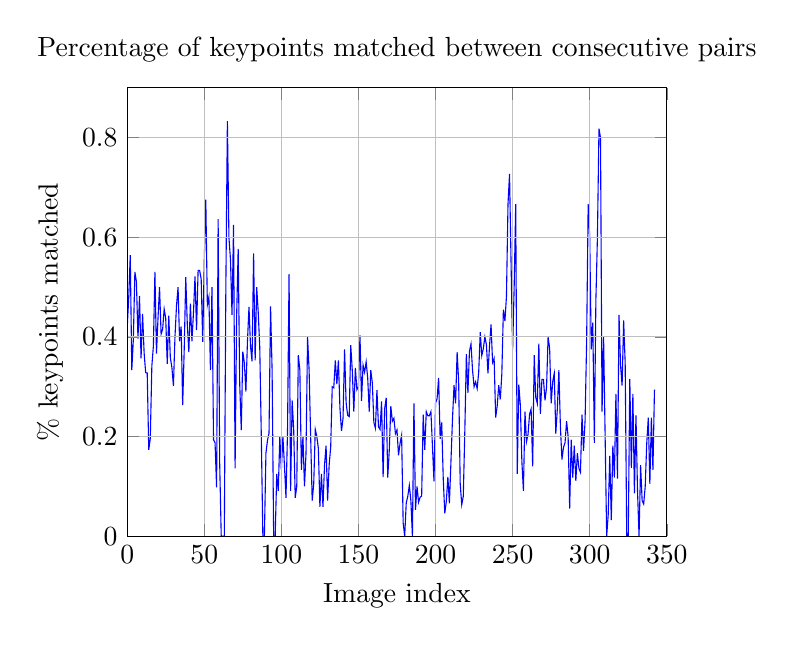
\begin{tikzpicture}

\begin{axis}[
title={Percentage of keypoints matched between consecutive pairs},
xlabel={Image index},
ylabel={\% keypoints matched},
xmin=0, xmax=350,
ymin=0, ymax=0.9,
axis on top,
tick pos=both,
xmajorgrids,
ymajorgrids
]
\addplot [blue, forget plot]
table {%
0 0.416666666666667
1 0.478260869565217
2 0.564102564102564
3 0.333333333333333
4 0.394736842105263
5 0.530612244897959
6 0.51063829787234
7 0.396551724137931
8 0.482142857142857
9 0.357142857142857
10 0.446428571428571
11 0.36734693877551
12 0.328358208955224
13 0.327586206896552
14 0.173333333333333
15 0.196428571428571
16 0.341463414634146
17 0.381818181818182
18 0.530612244897959
19 0.366666666666667
20 0.4375
21 0.5
22 0.405797101449275
23 0.415384615384615
24 0.455882352941176
25 0.4375
26 0.346153846153846
27 0.442622950819672
28 0.358208955223881
29 0.338983050847458
30 0.301587301587302
31 0.4
32 0.462686567164179
33 0.5
34 0.391304347826087
35 0.421052631578947
36 0.263157894736842
37 0.375
38 0.52
39 0.425
40 0.369565217391304
41 0.466666666666667
42 0.391304347826087
43 0.448275862068966
44 0.521739130434783
45 0.413793103448276
46 0.533333333333333
47 0.533333333333333
48 0.516129032258065
49 0.390243902439024
50 0.552631578947368
51 0.675675675675676
52 0.464285714285714
53 0.48
54 0.333333333333333
55 0.5
56 0.193548387096774
57 0.1875
58 0.0980392156862745
59 0.636363636363636
60 0.147058823529412
61 0
62 0
63 0
64 0.5
65 0.833333333333333
66 0.6
67 0.555555555555556
68 0.444444444444444
69 0.625
70 0.136363636363636
71 0.441860465116279
72 0.576923076923077
73 0.305555555555556
74 0.213114754098361
75 0.37037037037037
76 0.347826086956522
77 0.290322580645161
78 0.38961038961039
79 0.46031746031746
80 0.380952380952381
81 0.350877192982456
82 0.567567567567568
83 0.352941176470588
84 0.5
85 0.45
86 0.378378378378378
87 0.2
88 0
89 0
90 0.166666666666667
91 0.192307692307692
92 0.206896551724138
93 0.461538461538462
94 0.333333333333333
95 0
96 0
97 0.125
98 0.0909090909090909
99 0.2
100 0.133333333333333
101 0.2
102 0.142857142857143
103 0.0769230769230769
104 0.210526315789474
105 0.526315789473684
106 0.0909090909090909
107 0.272727272727273
108 0.214285714285714
109 0.0769230769230769
110 0.1
111 0.363636363636364
112 0.333333333333333
113 0.133333333333333
114 0.2
115 0.1
116 0.166666666666667
117 0.4
118 0.333333333333333
119 0.2
120 0.0714285714285714
121 0.105263157894737
122 0.214285714285714
123 0.2
124 0.176470588235294
125 0.0588235294117647
126 0.125
127 0.0588235294117647
128 0.142857142857143
129 0.181818181818182
130 0.0714285714285714
131 0.142857142857143
132 0.178571428571429
133 0.3
134 0.297872340425532
135 0.352941176470588
136 0.305084745762712
137 0.352941176470588
138 0.257142857142857
139 0.211267605633803
140 0.236111111111111
141 0.375
142 0.268292682926829
143 0.242857142857143
144 0.24
145 0.383561643835616
146 0.333333333333333
147 0.25
148 0.337837837837838
149 0.294117647058824
150 0.3
151 0.402985074626866
152 0.271428571428571
153 0.343283582089552
154 0.329113924050633
155 0.35
156 0.318181818181818
157 0.25
158 0.333333333333333
159 0.307692307692308
160 0.228571428571429
161 0.216867469879518
162 0.293333333333333
163 0.219512195121951
164 0.214285714285714
165 0.270588235294118
166 0.118421052631579
167 0.25609756097561
168 0.277777777777778
169 0.117647058823529
170 0.172839506172839
171 0.260869565217391
172 0.230769230769231
173 0.236842105263158
174 0.205882352941176
175 0.213333333333333
176 0.162162162162162
177 0.186666666666667
178 0.20253164556962
179 0.0266666666666667
180 0
181 0.0666666666666667
182 0.08
183 0.102040816326531
184 0.0714285714285714
185 0
186 0.266666666666667
187 0.0526315789473684
188 0.1
189 0.0681818181818182
190 0.078125
191 0.0804597701149425
192 0.24390243902439
193 0.173333333333333
194 0.25
195 0.241758241758242
196 0.241758241758242
197 0.25
198 0.180722891566265
199 0.11
200 0.267326732673267
201 0.275862068965517
202 0.317647058823529
203 0.195402298850575
204 0.228571428571429
205 0.115384615384615
206 0.0459770114942529
207 0.0697674418604651
208 0.119047619047619
209 0.0657894736842105
210 0.15
211 0.235294117647059
212 0.303030303030303
213 0.266666666666667
214 0.369565217391304
215 0.311111111111111
216 0.105263157894737
217 0.0632911392405063
218 0.08
219 0.211538461538462
220 0.365384615384615
221 0.287878787878788
222 0.371428571428571
223 0.385714285714286
224 0.333333333333333
225 0.3
226 0.309859154929577
227 0.296296296296296
228 0.329411764705882
229 0.409638554216867
230 0.3625
231 0.376623376623377
232 0.4
233 0.384615384615385
234 0.326923076923077
235 0.380952380952381
236 0.425
237 0.348837209302326
238 0.357142857142857
239 0.238095238095238
240 0.261904761904762
241 0.303030303030303
242 0.274509803921569
243 0.325581395348837
244 0.454545454545455
245 0.431818181818182
246 0.481481481481481
247 0.666666666666667
248 0.727272727272727
249 0.545454545454545
250 0.375
251 0.5
252 0.666666666666667
253 0.125
254 0.304347826086957
255 0.263157894736842
256 0.15
257 0.0909090909090909
258 0.25
259 0.189655172413793
260 0.204545454545455
261 0.245614035087719
262 0.25531914893617
263 0.140350877192982
264 0.363636363636364
265 0.278688524590164
266 0.266666666666667
267 0.386363636363636
268 0.245614035087719
269 0.314814814814815
270 0.314814814814815
271 0.272727272727273
272 0.298245614035088
273 0.4
274 0.377358490566038
275 0.266666666666667
276 0.310344827586207
277 0.326923076923077
278 0.205882352941176
279 0.255813953488372
280 0.333333333333333
281 0.21875
282 0.153846153846154
283 0.178571428571429
284 0.1875
285 0.230769230769231
286 0.2
287 0.0555555555555556
288 0.193548387096774
289 0.117647058823529
290 0.181818181818182
291 0.111111111111111
292 0.166666666666667
293 0.136363636363636
294 0.128205128205128
295 0.24390243902439
296 0.171428571428571
297 0.232558139534884
298 0.391304347826087
299 0.666666666666667
300 0.6
301 0.375
302 0.428571428571429
303 0.1875
304 0.473684210526316
305 0.6
306 0.818181818181818
307 0.8
308 0.25
309 0.4
310 0.2
311 0
312 0.0434782608695652
313 0.161290322580645
314 0.032258064516129
315 0.181818181818182
316 0.117647058823529
317 0.285714285714286
318 0.115384615384615
319 0.444444444444444
320 0.342857142857143
321 0.302325581395349
322 0.433333333333333
323 0.347826086956522
324 0
325 0
326 0.315789473684211
327 0.137254901960784
328 0.285714285714286
329 0.0857142857142857
330 0.242424242424242
331 0.0909090909090909
332 0
333 0.142857142857143
334 0.0714285714285714
335 0.0645161290322581
336 0.1
337 0.1875
338 0.238095238095238
339 0.105263157894737
340 0.238095238095238
341 0.133333333333333
342 0.294117647058824
};
\end{axis}

\end{tikzpicture}}
\caption{Plot of the percentage of keypoints matched between consecutive image pairs.}
\label{fig:tamu-fig3}
\end{figure}

Contrary to the other metrics which are true distances, a dip can be seen in both metrics around the anomalous images.
The average time for BRIEF extraction for a single image is 0.244 seconds.
Distance metric calculation is a single operation of negligible processing time.

\subsection{Blob Detection}

Below are figures showing the difference in number of blobs (figure 3.6) and the difference in total blob area (figure 3.7) between consecutive image pairs.

\begin{figure}[htb]
\centering
\scalebox{1.0}{% This file was created by matplotlib2tikz v0.6.11.
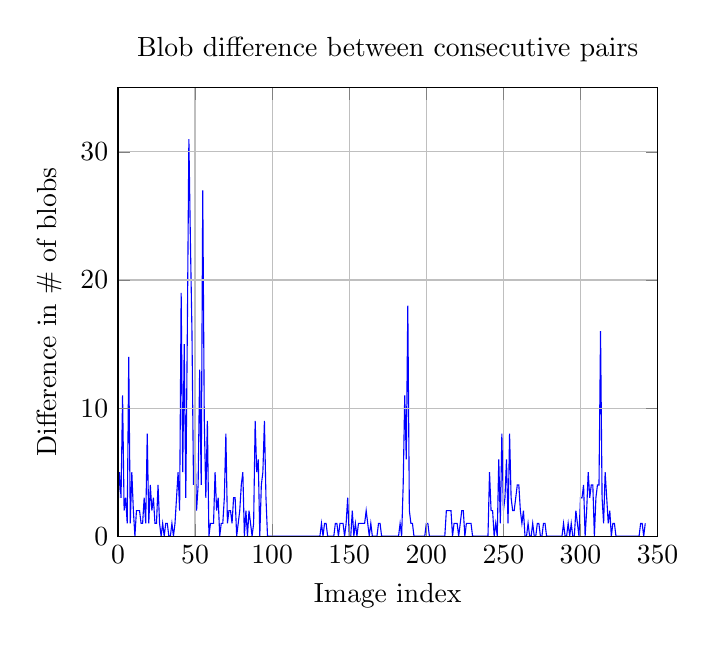
\begin{tikzpicture}

\begin{axis}[
title={Blob difference between consecutive pairs},
xlabel={Image index},
ylabel={Difference in \# of blobs},
xmin=0, xmax=350,
ymin=0, ymax=35,
axis on top,
tick pos=both,
xmajorgrids,
ymajorgrids
]
\addplot [blue, forget plot]
table {%
0 2
1 5
2 3
3 11
4 2
5 3
6 1
7 14
8 1
9 5
10 2
11 0
12 2
13 2
14 2
15 1
16 1
17 3
18 1
19 8
20 1
21 4
22 2
23 3
24 1
25 1
26 4
27 1
28 0
29 1
30 0
31 1
32 1
33 0
34 0
35 1
36 0
37 1
38 3
39 5
40 2
41 19
42 5
43 15
44 3
45 16
46 31
47 23
48 16
49 4
50 7
51 2
52 4
53 13
54 4
55 27
56 9
57 3
58 9
59 0
60 1
61 1
62 1
63 5
64 2
65 3
66 0
67 1
68 1
69 3
70 8
71 1
72 2
73 2
74 1
75 3
76 3
77 0
78 1
79 2
80 4
81 5
82 0
83 2
84 0
85 2
86 1
87 0
88 1
89 9
90 5
91 6
92 0
93 4
94 5
95 9
96 3
97 0
98 0
99 0
100 0
101 0
102 0
103 0
104 0
105 0
106 0
107 0
108 0
109 0
110 0
111 0
112 0
113 0
114 0
115 0
116 0
117 0
118 0
119 0
120 0
121 0
122 0
123 0
124 0
125 0
126 0
127 0
128 0
129 0
130 0
131 0
132 1
133 0
134 1
135 1
136 0
137 0
138 0
139 0
140 0
141 1
142 1
143 0
144 1
145 1
146 1
147 0
148 1
149 3
150 0
151 0
152 2
153 0
154 1
155 0
156 1
157 1
158 1
159 1
160 1
161 2
162 1
163 0
164 1
165 0
166 0
167 0
168 0
169 1
170 1
171 0
172 0
173 0
174 0
175 0
176 0
177 0
178 0
179 0
180 0
181 0
182 0
183 1
184 0
185 4
186 11
187 6
188 18
189 2
190 1
191 1
192 0
193 0
194 0
195 0
196 0
197 0
198 0
199 0
200 1
201 1
202 0
203 0
204 0
205 0
206 0
207 0
208 0
209 0
210 0
211 0
212 0
213 2
214 2
215 2
216 2
217 0
218 1
219 1
220 1
221 0
222 1
223 2
224 2
225 0
226 1
227 1
228 1
229 1
230 0
231 0
232 0
233 0
234 0
235 0
236 0
237 0
238 0
239 0
240 0
241 5
242 2
243 2
244 0
245 1
246 0
247 6
248 1
249 8
250 2
251 3
252 6
253 1
254 8
255 3
256 2
257 2
258 3
259 4
260 4
261 2
262 1
263 2
264 0
265 0
266 1
267 0
268 0
269 1
270 0
271 0
272 1
273 1
274 0
275 0
276 1
277 1
278 0
279 0
280 0
281 0
282 0
283 0
284 0
285 0
286 0
287 0
288 0
289 1
290 0
291 0
292 1
293 0
294 1
295 0
296 0
297 2
298 1
299 0
300 3
301 3
302 4
303 0
304 2
305 5
306 3
307 4
308 4
309 0
310 3
311 4
312 4
313 16
314 3
315 1
316 5
317 3
318 1
319 2
320 0
321 1
322 1
323 0
324 0
325 0
326 0
327 0
328 0
329 0
330 0
331 0
332 0
333 0
334 0
335 0
336 0
337 0
338 0
339 1
340 1
341 0
342 1
};
\end{axis}

\end{tikzpicture}}
\caption{Plot of the difference in number of blobs between consecutive image pairs.}
\label{fig:tamu-fig3}
\end{figure}



\begin{figure}[htb]
\centering
\scalebox{1.0}{% This file was created by matplotlib2tikz v0.6.11.
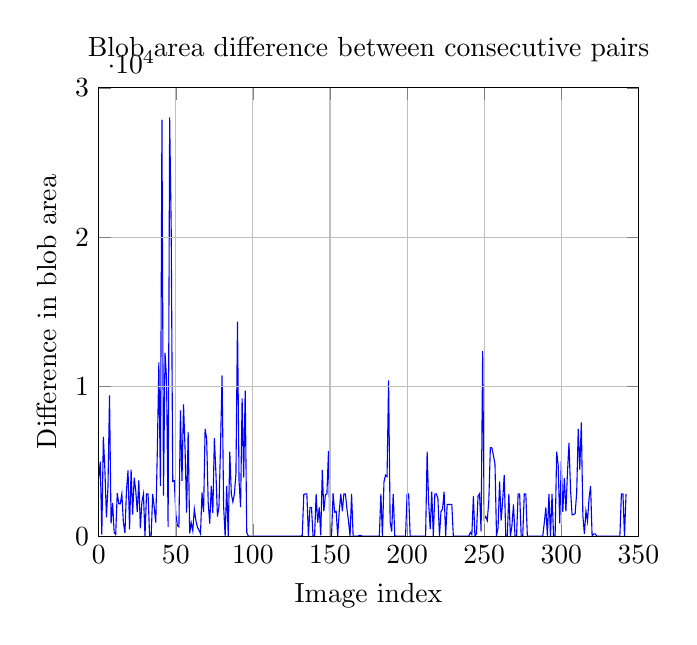
\begin{tikzpicture}

\begin{axis}[
title={Blob area difference between consecutive pairs},
xlabel={Image index},
ylabel={Difference in blob area},
xmin=0, xmax=350,
ymin=0, ymax=30000,
axis on top,
tick pos=both,
xmajorgrids,
ymajorgrids
]
\addplot [blue, forget plot]
table {%
0 3839.02622268673
1 4982.56594859341
2 97.3893722612847
3 6657.03483295677
4 4435.92882686879
5 1253.49546878233
6 3298.67228626928
7 9427.91955342297
8 851.371609122833
9 2221.10600608798
10 260.752190247953
11 103.672557568463
12 2877.69887068825
13 2173.98211628414
14 2173.98211628414
15 2827.43338823081
16 907.92027688745
17 213.628300444106
18 3075.61920786441
19 4401.3713076793
20 458.672527424113
21 4461.06156809751
22 1438.84943534413
23 3917.56603902647
24 3072.47761521082
25 1605.35384598438
26 3735.35366511826
27 530.929158456675
28 2296.50422977414
29 2827.43338823081
30 0
31 2827.43338823081
32 2827.43338823081
33 0
34 0
35 2827.43338823081
36 1919.51311134336
37 907.92027688745
38 5705.13225891906
39 11623.8928182822
40 3370.92891730185
41 27869.068429995
42 2717.47764535516
43 12264.7777196146
44 10530.618574833
45 631.460123371573
46 28023.006470021
47 20555.440732438
48 3659.95544143211
49 3713.36251654313
50 1482.83173249438
51 703.716754404104
52 622.035345410772
53 8425.75149692783
54 3694.5129606216
55 8821.59217128014
56 5811.94640914112
57 1570.7963267949
58 6983.76046893011
59 194.778744522566
60 885.929128312324
61 361.283155162824
62 1812.69896112131
63 1049.29194629899
64 600.04419683565
65 420.973415581032
66 166.50441064026
67 2921.68116783851
68 1605.35384598438
69 7184.82239875986
70 6509.37997823805
71 2246.2387473167
72 845.088423815654
73 3358.36254668749
74 1548.80517821977
75 6562.78705334907
76 4266.28282357494
77 1319.46891450771
78 1982.34496441516
79 6082.12337734984
80 10759.954838545
81 2004.33611299029
82 0
83 3358.36254668749
84 0
85 5654.86677646163
86 2827.43338823081
87 2296.50422977414
88 2827.43338823081
89 4216.0173411175
90 14360.2200195589
91 3691.37136796801
92 1954.07063053286
93 9223.71603093963
94 3920.70763168006
95 9742.07881878195
96 254.469004940773
97 0
98 0
99 0
100 0
101 0
102 0
103 0
104 0
105 0
106 0
107 0
108 0
109 0
110 0
111 0
112 0
113 0
114 0
115 0
116 0
117 0
118 0
119 0
120 0
121 0
122 0
123 0
124 0
125 0
126 0
127 0
128 0
129 0
130 0
131 0
132 50.2654824574367
133 2777.16790577338
134 2827.43338823081
135 2827.43338823081
136 0
137 1919.51311134336
138 1919.51311134336
139 0
140 0
141 2827.43338823081
142 907.92027688745
143 1919.51311134336
144 50.2654824574365
145 4439.07041952238
146 1661.902513749
147 2777.16790577338
148 2827.43338823081
149 5705.13225891906
150 0
151 0
152 2877.69887068825
153 1611.63703129156
154 1661.902513749
155 0
156 1661.902513749
157 2827.43338823081
158 1661.902513749
159 2827.43338823081
160 2827.43338823081
161 1815.8405537749
162 1011.59283445591
163 0
164 2827.43338823081
165 0
166 0
167 0
168 0
169 50.2654824574367
170 50.2654824574367
171 0
172 0
173 0
174 0
175 0
176 0
177 0
178 0
179 0
180 0
181 0
182 0
183 2827.43338823081
184 0
185 3631.6811075498
186 4080.92885701314
187 3989.82267005904
188 10430.0876099181
189 958.185759344887
190 314.159265358979
191 2827.43338823081
192 0
193 0
194 0
195 0
196 0
197 0
198 0
199 0
200 2827.43338823081
201 2827.43338823081
202 0
203 0
204 0
205 0
206 0
207 0
208 0
209 0
210 0
211 0
212 0
213 5654.86677646163
214 2195.97326485927
215 477.522083345648
216 2981.37142825671
217 0
218 2827.43338823081
219 2827.43338823081
220 2519.55730817901
221 0
222 1661.902513749
223 1815.8405537749
224 2981.37142825671
225 0
226 2123.7166338267
227 2123.7166338267
228 2123.7166338267
229 2123.7166338267
230 0
231 0
232 0
233 0
234 0
235 0
236 0
237 0
238 0
239 0
240 0
241 251.327412287183
242 100.530964914873
243 2676.6369408585
244 0
245 153.9380400259
246 2673.49534820491
247 2846.28294415235
248 314.15926535898
249 12387.2998331046
250 1149.82291121386
251 1319.46891450771
252 1046.1503536454
253 2362.47767549953
254 5921.90215201676
255 5912.47737405599
256 5397.25617886727
257 4831.7695012211
258 56.5486677646149
259 552.920307031804
260 3666.23862673929
261 1039.86716833822
262 2422.16793591773
263 4084.07044966673
264 0
265 0
266 2827.43338823081
267 0
268 703.716754404114
269 2123.7166338267
270 0
271 0
272 2827.43338823081
273 2827.43338823081
274 0
275 0
276 2827.43338823081
277 2827.43338823081
278 0
279 0
280 0
281 0
282 0
283 0
284 0
285 0
286 0
287 0
288 0
289 907.92027688745
290 1919.51311134336
291 0
292 2827.43338823081
293 0
294 2827.43338823081
295 0
296 0
297 5654.86677646163
298 4746.94649957418
299 857.654794430014
300 5001.41550451495
301 1627.34499455951
302 3876.7253345298
303 1655.61932844182
304 4222.30052642468
305 6242.34460268292
306 3125.88469032184
307 1426.28306472977
308 1448.2742133049
309 1507.9644737231
310 2927.96435314569
311 7172.2560281455
312 4451.63679013674
313 7608.93740699448
314 1376.01758227233
315 153.9380400259
316 1683.89366232413
317 999.026463841554
318 2519.55730817901
319 3358.36254668749
320 0
321 153.9380400259
322 153.9380400259
323 0
324 0
325 0
326 0
327 0
328 0
329 0
330 0
331 0
332 0
333 0
334 0
335 0
336 0
337 0
338 0
339 2827.43338823081
340 2827.43338823081
341 0
342 2827.43338823081
};
\end{axis}

\end{tikzpicture}}
\caption{Plot of the difference in total blob area between consecutive image pairs.}
\label{fig:tamu-fig3}
\end{figure}

Similarly to the distribution distance plots, spikes can be seen around the anomalous images, as well as in other places.
The average time for extraction of blobs for a single image is 1.06 seconds -- the longest time for any of the considered features.

\section{Learning Algorithm Evaluation}

To evaluate the learning algorithms, these distance metrics were concatenated into feature vectors, and fed along with the corresponding label vector to train each algorithm.
As stated in the testing methodology, the models were then tuned to increase performance, and the final averaged values for detection rate, false alarm rate, and overall accuracy are reported in the table below:

\begin{table}[h!]
	\centering
	\begin{tabular}{|l|l|l|l|}
		\hline
		Algorithm & Detection Rate & False Alarm Rate & Overall Accuracy  \\ \hline
		Logistic Regression & 0.956 & 0.077 & 0.933  \\ \hline
		Decision Trees & 0.119 & 0.033 & 0.899  \\ \hline
		Neural Network & 0.75 & 0.038 & 0.959  \\ \hline
		SVM & 0.924 & 0.258  & 0.743 \\ \hline
	\end{tabular}
	\caption{Performance of learning algorithms in anomalous image detection}
\end{table}


The logistic regression model performed the best out of the four algorithms with a 95.6\% detection rate and a 7.7\% false positive rate.
The decision tree predictably performed poorly, as it is a simple model incapable of considering the interaction between features.
The SVM and neural network had decent performance, with the neural network missing 25\% of anomalous image pairs, and the SVM having a fairly high false alarm rate of 25.8\%.

% \section{Yet Another Table}

% Another table is placed here to show the effect of having tables in multiple sections. The list of tables should still double space between table titles, while single spacing long table titles.

% %Fix table labeling.
% \begin{table}[h!]
% 	\centering
% 	\begin{tabular}{|l|l|}
% 		\hline
% 		Dates & Attendance  \\ \hline
% 		August 8-10, 2008 & 3,523  \\ \hline
% 		August 14-16, 2009 & 4,003 \\ \hline
% 		July 9-11, 2010 & 5,049 \\ \hline
% 		August 5-7, 2011 & 6,891  \\ \hline
% 		August 10-12, 2012 & 9,464  \\ \hline
% 		August 16-18, 2013 & 11,077  \\ \hline
% 		July 18-20, 2014 & 14,686 \\ \hline
% 		July 31-August 2, 2015 & 18,411  \\ \hline
% 	\end{tabular}
% 	\caption{San Japan attendance. Data is taken from \cite{ANCONS}. I intentionally make the title of this table long so the single space effect is seen in the list of tables.}
% \end{table}

% You may be wondering why San Japan was chosen. There are a few reasons as to why I did this:

% \begin{enumerate}
% \item It is one of the fastest-growing anime conventions in Texas.
% \item Filler.
% \item I wanted a good variety of table examples.
% \item Because conventions are cool.
% \end{enumerate}


